\section{Exact robustification under product geometric uncertainty}
\label{sec:uncertainty}
The usual margin bound gives sufficient protection against geometric errors. In a product uncertainty model one can do better: the robust coverage region has an exact reduction. This is a worst-case statement about possible placements, with no probability distribution assumed.

Let contact $i$ have a family of possible closed footprints $D_i(\theta_i)$ indexed by a nonempty set $\Theta_i$. The complete uncertainty set is
\[
\Theta=\prod_{i=1}^n\Theta_i.
\]
Define the footprint guaranteed for every local parameter by
\begin{equation}\label{eq:guaranteed-footprint}
E_i=\bigcap_{\theta_i\in\Theta_i}D_i(\theta_i).
\end{equation}
The fault rule $w$ is fixed on the contact labels and does not depend on the realized parameters.

\begin{theorem}[Product uncertainty commutes with monotone logic]\label{thm:product}
For every monotone winning rule $w$ and every point $x$,
\begin{equation}\label{eq:product-logic}
\begin{aligned}
&w(S_\theta(x))=1\text{ for every }\theta\in\Theta\\
&\quad\Longleftrightarrow\quad w(\{i:x\in E_i\})=1.
\end{aligned}
\end{equation}
Consequently the region covered under the rule for every allowed geometric realization is exactly the winning region of the guaranteed footprints. In particular,
\begin{equation}\label{eq:product-target}
\forall\theta\in\Theta\quad T\subseteq R_w(D(\theta))
\quad\Longleftrightarrow\quad T\subseteq R_w(E).
\end{equation}
\end{theorem}
\begin{proof}
Write $I(x)=\{i:x\in E_i\}$. Every active set $S_\theta(x)$ contains $I(x)$, so a winning $I(x)$ gives the left side by monotonicity. Conversely, if $i\notin I(x)$, choose one local parameter $\theta_i$ for which $x\notin D_i(\theta_i)$. Choose arbitrary parameters for the other contacts. The product hypothesis permits all those local choices simultaneously. Their resulting active set is exactly $I(x)$. Thus the left side requires that this set wins. This proves \cref{eq:product-logic}. Finally, universal quantifiers over the target point and the parameter realization commute, giving \cref{eq:product-target}.
\end{proof}

The proof is a statement about an attainable least active set. It is not an unjustified exchange of an intersection and a union. Compactness and convexity are unnecessary for the logical theorem, although they are useful for computing the guaranteed footprints.\footnote{The adversarial realization used to disprove full-target coverage may depend on the exhibited point. This is legitimate: failure of a statement quantified over all realizations and all target points requires one pair consisting of a realization and a point.}

\subsection{Independent displacement balls and radius intervals}
Suppose the center of contact $i$ is $c_i+u_i$, with $\|u_i\|\le\epsilon_i$, and its radius lies in an interval $[\underline r_i,\overline r_i]$ with $\underline r_i\ge0$. Parameters for distinct contacts may be chosen independently. The largest distance from $x$ to a possible center is
\[
\sup_{\|u_i\|\le\epsilon_i}\|x-c_i-u_i\|=\|x-c_i\|+\epsilon_i.
\]
The upper bound is the triangle inequality. Equality follows by taking the displacement directly away from $x$, or any direction when $x=c_i$.

\begin{corollary}[Exact erosion]\label{cor:erosion}
The guaranteed footprint is the closed disk of radius $\underline r_i-\epsilon_i$ centered at $c_i$ when this radius is nonnegative, and is empty otherwise. Coverage of the eroded family is necessary and sufficient for robust full-target coverage under every fixed monotone failure rule.
\end{corollary}
\begin{proof}
Membership in $E_i$ is exactly the inequality $\|x-c_i\|+\epsilon_i\le\underline r_i$. Apply \cref{thm:product}.
\end{proof}

When $\underline r_i=\epsilon_i$, the footprint is a point rather than an empty set. The algorithm preserves the distinction, although isolated footprint points cannot rescue a positive-area target that fails on an open subset. An empty guaranteed footprint is represented by an always-inactive contact, not by a disk with a negative radius.

\begin{corollary}[Exact common-radius uncertainty allowance]\label{cor:radius-error}
If all nominal radii equal $r_0$, all downward radius errors are at most $\eta$ and all independent displacement balls have radius $\epsilon$, with $r_0\ge\eta$, robust coverage holds exactly when
\[
r_0-\eta-\epsilon\ge r_w^*.
\]
If $r_0-\eta\ge r_w^*$, the maximum allowed independent displacement radius is $r_0-\eta-r_w^*$. The threshold $r_w^*$ is supplied by \cref{thm:master-radius}.
\end{corollary}

The equality is exact for the product model. It is stronger than using a Lipschitz estimate only in the sufficient direction. For unequal errors, the eroded radii may differ; the exact fixed-radius target algorithm remains applicable even though the common-radius bisector theorem no longer has that form.

\subsection{Independent polygonal displacement uncertainty}
Suppose $u_i$ ranges over the convex hull of a finite rational set $V_i$. For fixed $x$ and any convex combination $u=\sum_v\lambda_v v$,
\[
\|x-c_i-u\|\le\sum_v\lambda_v\|x-c_i-v\|
\le\max_{v\in V_i}\|x-c_i-v\|.
\]
The reverse inequality for the supremum holds because the vertices themselves are allowed. Therefore
\begin{equation}\label{eq:uncertainty-bundle}
E_i=\bigcap_{v\in V_i}\overline B(c_i+v,\underline r_i).
\end{equation}

\begin{theorem}[Finite primitive-disk reduction]\label{thm:bundle}
For product polygonal displacement uncertainty, introduce one primitive disk for every shifted center in \cref{eq:uncertainty-bundle}. A physical contact is active exactly when every primitive disk in its bundle is active. Applying that monotone bundle map to the primitive target antichain gives an exact robust target certificate for every failure family on the physical contacts. If the lower radii are common, the same bundle map can be used in the exact common-radius theorem.
\end{theorem}
\begin{proof}
\Cref{eq:uncertainty-bundle} proves the bundle activation statement. \Cref{thm:relabel} gives its target antichain, and \cref{thm:product} identifies the robust region. With common radii, the winning predicate on primitive sets is the composition of the monotone physical rule and the monotone bundle map. It meets the hypotheses of \cref{thm:master-radius} when the full primitive set wins.
\end{proof}

There are $N=\sum_i|V_i|$ primitive disks. The target certificate-size bound uses $N$ in place of the number of physical contacts. This is an exact vertex reduction of the stated uncertainty polytope, not an approximation of a displacement ball by a polygon. For independent boxes, four corner disks per physical contact suffice in the plane.

\begin{proposition}[Robust convex nerve models]\label{prop:bundle-nerve}
The guaranteed footprints in \cref{eq:uncertainty-bundle} are closed convex sets. Their maximal nerve faces are obtained by applying the bundle activation map to the maximal primitive-disk nerve faces and retaining maximal images. Thus the topological models in \cref{sec:duality} also apply to the robust region, with at most $N^2$ maximal faces from the primitive witness bound.
\end{proposition}
\begin{proof}
The guaranteed footprints are finite intersections of disks. Every realized primitive mask is contained in a maximal primitive nerve face. Monotonicity of the bundle map sends this containment to containment of physical masks. Every maximal primitive face is realized at a point, so its image is also realized. Taking maximal images therefore gives exactly the maximal physical masks. Each physical nerve face is contained in one of these maximal masks. Apply \cref{thm:witness,thm:duality}.
\end{proof}

For arbitrary monotone activation using disjunctions, target relabeling remains correct, but the resulting physical footprints need not be convex. The classical convex nerve equivalence then requires separate good-cover hypotheses. The target certificate does not silently inherit that extra topological assertion.

\subsection{A counterexample for shared placement errors}
The product hypothesis cannot be dropped. Put nominal centers at $(\pm3/5,0)$, give both disks radius $1$ and let them share one displacement vector $u$ with $\|u\|\le3/5$. At the origin,
\[
\min_{\pm}\|u\pm(3/5,0)\|^2
=\|u\|^2+9/25-(6/5)|u_x|\le18/25.
\]
Every point of the square $[-1/10,1/10]^2$ is within $\sqrt2/10$ of the origin, so its distance to at least one shifted center is at most
\[
\sqrt{18/25}+\sqrt2/10=7\sqrt2/10<1.
\]
The shared-error model therefore covers the whole square for every $u$. Eroding each nominal disk independently by $3/5$ gives radius $2/5$ and leaves the origin uncovered. That eroded test is sufficient but is not necessary for this shared-error support. Under genuinely independent errors, choosing opposite outward shifts would uncover the origin, exactly as \cref{thm:product} predicts.

Fault-domain correlation and geometric correlation are different inputs. The failure family may correlate contact losses arbitrarily in \cref{thm:product}; the theorem restricts the support of the geometric parameters. Statistical independence is not a substitute for stating that support. These distinctions are central to applying robust optimization correctly~\cite{robustbook}.

\begin{figure*}[tb]
\centering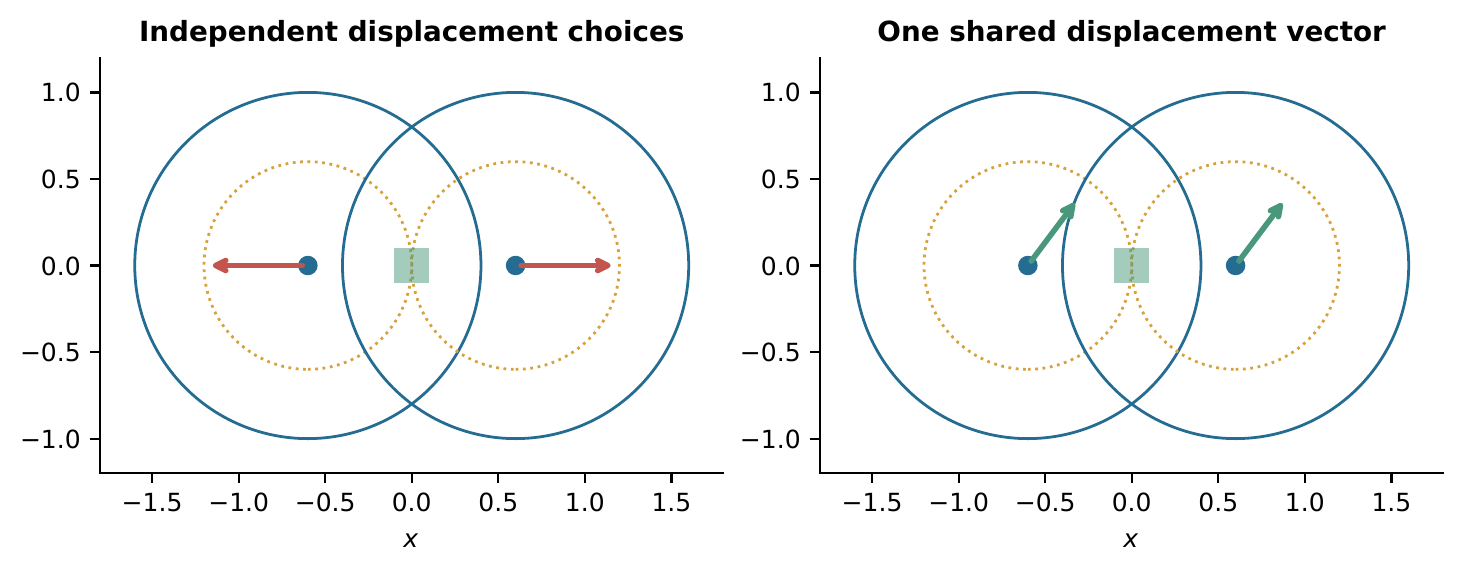
\includegraphics[width=\textwidth]{figures/product-errors.png}
\caption{The difference between product and shared geometric errors in the counterexample of \cref{sec:uncertainty}. Independent choices may move both disks outward. A shared displacement cannot make those opposite moves simultaneously.}
\end{figure*}

\begin{figure*}[tb]
\centering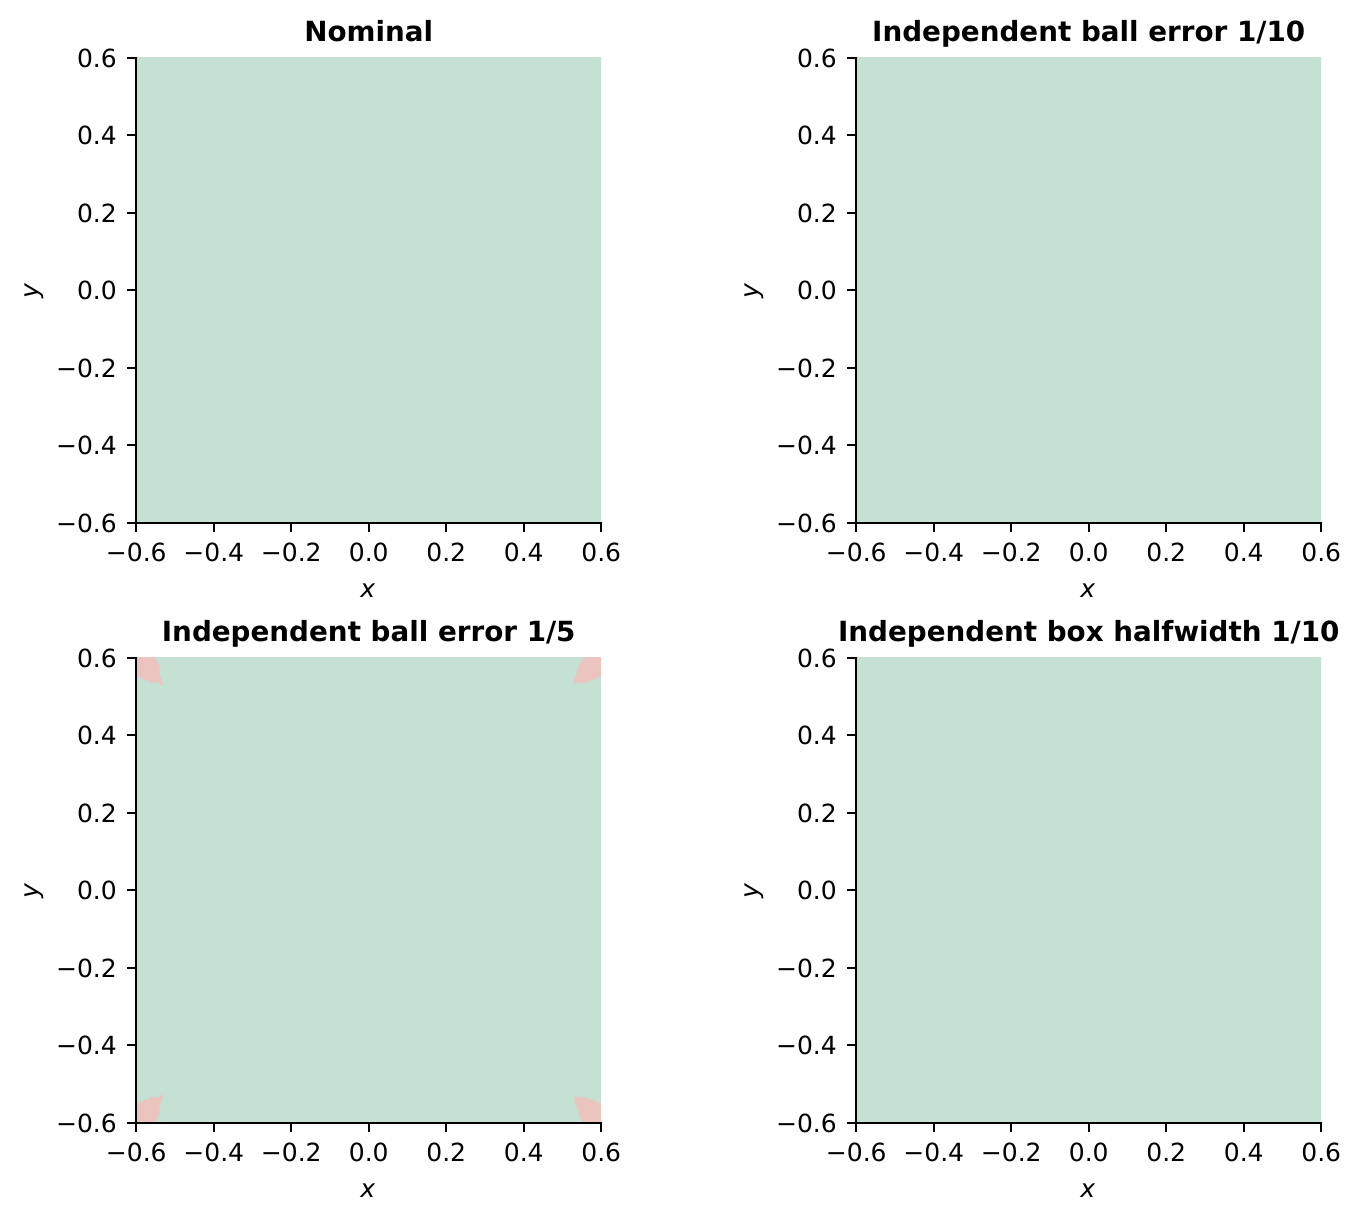
\includegraphics[width=.72\textwidth]{figures/uncertainty-panel.png}
\caption{Guaranteed two-contact target coverage under four placement models. Shading illustrates the winning region; exact target antichains and the support-radius certificate determine acceptance. The box model is represented by finite conjunction bundles, not by an unproved circular approximation.}
\end{figure*}

